\documentclass[border=10pt]{standalone}
\usepackage{pgfplots}
\pgfplotsset{compat=1.18}
\begin{document}
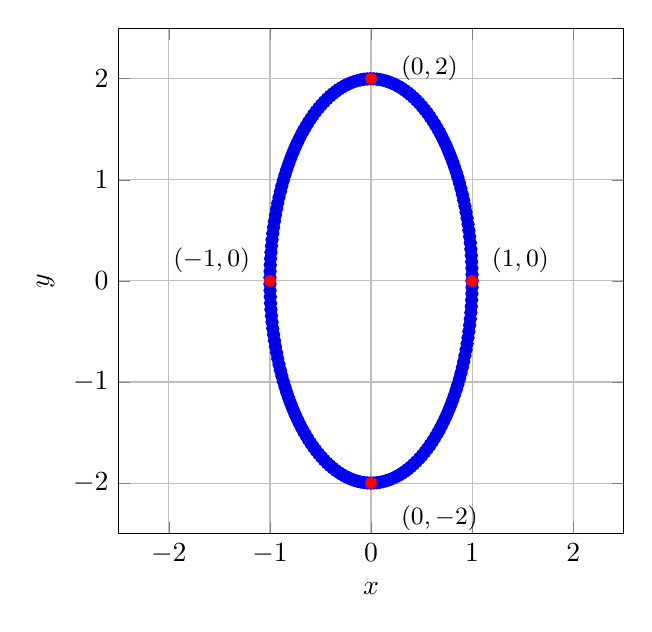
\begin{tikzpicture}
\begin{axis}[
    axis equal,
    xlabel={$x$},
    ylabel={$y$},
    grid=major,
    xmin=-2.5, xmax=2.5,
    ymin=-2.5, ymax=2.5,
    width=8cm,
    height=8cm
]
\addplot+[domain=0:360, samples=200, thick, blue] ({cos(x)}, {2*sin(x)});
\addplot[only marks, mark=*, red] coordinates {(1,0) (-1,0) (0,2) (0,-2)};
\node[anchor=west, font=\small] at (axis cs:1.1,0.2) {$(1,0)$};
\node[anchor=east, font=\small] at (axis cs:-1.1,0.2) {$(-1,0)$};
\node[anchor=west, font=\small] at (axis cs:0.2,2.1) {$(0,2)$};
\node[anchor=west, font=\small] at (axis cs:0.2,-2.35) {$(0,-2)$};
\end{axis}
\end{tikzpicture}
\end{document}